\documentclass[a4paper,fleqn]{cas-dc}

\usepackage[spanish,es-tabla,es-nodecimaldot]{babel}
\usepackage{csquotes}
\usepackage[backend=biber,style=apa]{biblatex}
\addbibresource{references.bib}
\usepackage{float}
\usepackage{xurl}
% cas-dc ya carga graphicx, amsmath, amssymb, booktabs y hyperref

% Permite varias figuras y tablas a dos columnas por página
\setcounter{dbltopnumber}{3}
\renewcommand{\dbltopfraction}{0.9}
\renewcommand{\dblfloatpagefraction}{0.8}
\graphicspath{{figures/}}
\hypersetup{
    linkcolor=blue,
    filecolor=magenta,
    urlcolor=cyan,
    citecolor=blue
}

% Localización de textos fijos de cas-dc
\ExplSyntaxOn
\RenewDocumentCommand \printorcid { } { } % evita la línea "ORCID(s):" vacía
\RenewDocumentEnvironment { keywords } { O{ Palabras~clave } }
   {
     \tex_global:D \tex_setbox:D \g_stm_key_box = \vtop \bgroup
     \hsize=.25 \textwidth
     \cs_set:Npn \sep { \par }
     \parindent = 0pt
     I\,N\,F\,O\,R\,M\,A\,C\,I\,Ó\,N \par \skip_vertical:n { -3pt }
     \rule{.25 \textwidth}{.2pt}\par\footnotesize
     \noindent \textit { #1 }:  \par
   }
   { \egroup }
\ExplSyntaxOff

\begin{document}
\let\WriteBookmarks\relax
\def\floatpagepagefraction{1}
\def\textpagefraction{.001}
\shorttitle{Clasificación automática de 104 tipos de flores}
\shortauthors{Eduardo-Luna et al.}

\title [mode = title]{Clasificación automática de 104 tipos de flores con redes neuronales profundas}
\tnotemark[1]
\tnotetext[1]{Situación problema: Avance 3 (versión corregida). Diseño de Redes Neuronales y Aprendizaje Profundo (TC2035.201). Proyecto basado en la competencia \textit{Petals to the Metal -- Flower Classification on TPU} de Kaggle. Código y notebook: \url{https://github.com/Lunaaaalj/NeuralNetworksTeamEnvironment}.}

\author[1]{Angel Eduardo-Luna}
\fnmark[1]
\author[1]{Andrea Estefanía De la Peña Contreras}
\fnmark[2]
\author[1]{Jannette Cristina Flores Rodríguez}
\fnmark[3]
\author[1]{Rey Iván de la Fuente Chávez}
\fnmark[4]
\author[1]{Andrés Huerta Robinson}
\fnmark[5]

\affiliation[1]{organization={Escuela de Ingeniería y Ciencias, Tecnológico de Monterrey},
    city={Monterrey},
    state={Nuevo León},
    country={México}}

\fntext[1]{Matrícula: A00842657}
\fntext[2]{Matrícula: A00840973}
\fntext[3]{Matrícula: A01255711}
\fntext[4]{Matrícula: A01709445}
\fntext[5]{Matrícula: A00838626}

\begin{abstract}
Este trabajo aborda la clasificación automática de 104 tipos de flores mediante redes neuronales convolucionales (CNN) y técnicas de destilación de datos. Se utiliza el conjunto de imágenes de la competencia \textit{Petals to the Metal} de Kaggle, compuesto por 23,847 fotografías RGB distribuidas entre entrenamiento, validación y prueba. La similitud visual entre algunas clases, las variaciones de iluminación y el desbalance de los datos representan desafíos importantes para la clasificación.

Se implementó una CNN de cuatro bloques convolucionales (480,936 parámetros), entrenada mediante retropropagación con el optimizador Adam, parada temprana por F1 macro y guardado del mejor modelo. Además, se aplicó \textit{Distribution Matching} (DM) para generar conjuntos reducidos de imágenes sintéticas, y se comparó el entrenamiento con el conjunto completo, con subconjuntos aleatorios de imágenes reales y con conjuntos destilados de una y diez imágenes por clase.

Con el conjunto completo, el modelo alcanzó un F1 macro de 0.5538 y una exactitud de 61.61\,\% en validación. Las curvas de aprendizaje muestran que, a partir de la época 25, la pérdida de validación se estanca mientras la de entrenamiento sigue bajando, y que los conjuntos reducidos memorizan sus pocas imágenes. Con el conjunto completo se evaluaron tres variaciones de hiperparámetros (tasa de aprendizaje, \textit{dropout} y regularización): reducir la tasa de aprendizaje a $3\times10^{-4}$ produjo subajuste (F1 de 0.4605) y quitar la regularización aumentó el sobreajuste (F1 de 0.5332), mientras que la configuración de referencia obtuvo el mejor F1, 0.5784. Todas las tablas y figuras se reproducen con el notebook público del proyecto.
\end{abstract}

\begin{keywords}
Clasificación de imágenes \sep
Redes neuronales convolucionales \sep
Curvas de aprendizaje \sep
Destilación de datos \sep
F1 macro
\end{keywords}


\maketitle

\section{Contexto del problema}
La diversidad del mundo natural es enorme: se estima que existen más de 5,000 especies de mamíferos, 10,000 de aves y 30,000 de peces, pero hay más de 400,000 tipos de flores \parencite{kagglePetalsMetal}. Distinguir entre ellas puede requerir conocimiento especializado y, aun para una persona con experiencia, muchas flores son visualmente muy parecidas entre sí. Identificarlas de forma manual es lento y no escala cuando se tienen miles de fotografías. Por eso resulta valioso contar con modelos que reconozcan el tipo de flor de forma automática a partir de una imagen.

Este proyecto parte de la competencia \textit{Petals to the Metal}, de Kaggle, cuyo reto es construir un modelo que identifique el tipo de flor en un conjunto de imágenes. La competencia se limita a 104 clases de flores y consiste en un problema de clasificación multiclase de imágenes en el que el modelo debe captar detalles finos de forma, estructura y color para distinguir entre categorías cercanas.

Este problema tiene varias dificultades que lo hacen relevante desde un enfoque de redes neuronales. Primero, las clases son heterogéneas, ya que algunas solo tienen un subtipo de flor y otras agrupan muchas subvariedades. Además, las imágenes no fueron capturadas en el mismo entorno, lo que les da más variedad. Por último, el número de imágenes por clase tampoco es uniforme, por lo que, considerando la métrica de evaluación, es importante que el modelo funcione bien tanto en las clases con pocos ejemplos como en las que tienen muchos.

\section{Descripción del dataset}
\subsection{Origen}
Los datos vienen de \textit{Petals to the Metal -- Flower Classification on TPU}, una competencia \textit{Getting Started} de Kaggle cuyo objetivo es aprender a entrenar modelos en TPU \parencite{kagglePetalsMetal}. Según la descripción de la competencia, las imágenes se tomaron de cinco conjuntos de datos públicos. Algunas clases son muy específicas (por ejemplo, \textit{pink primrose}, que contiene un solo subtipo de flor) y otras agrupan muchas subvariedades (por ejemplo, \textit{wild rose}).

Al revisar la lista de clases nos dimos cuenta de que las primeras 102 siguen exactamente el orden del conjunto Oxford 102 Flowers \parencite{nilsback2008}: 94 conservan el mismo nombre y las otras 8 se renombraron, se corrigieron o se ampliaron (por ejemplo, \textit{oxeye daisy} pasó a ser \textit{daisy} y \textit{bearded iris} pasó a ser \textit{iris}). Las dos clases extra son \textit{common tulip} y \textit{wild rose}. Las etiquetas están en inglés, así que usamos los nombres originales en cursiva.

\subsection{Tamaño y estructura}
En total hay 23,847 imágenes a color (RGB) de 104 clases, repartidas como muestra la Tabla~\ref{tab:particiones}. Vienen en formato TFRecord, que junta muchas imágenes en pocos archivos binarios para que la TPU las lea rápido. Cada registro tiene tres campos: \texttt{image} (la foto codificada en JPEG), \texttt{id} (un identificador único) y \texttt{class} (la etiqueta, un entero de 0 a 103). Los registros de prueba no traen \texttt{class}, porque esas etiquetas solo las tiene Kaggle para calificar.

\begin{table}[htbp]
\centering
\caption{Particiones del conjunto de datos.}
\label{tab:particiones}
\small
\begin{tabular}{lrrc}
\toprule
Partición & Imágenes & \% & ¿Etiquetado? \\
\midrule
Entrenamiento & 12,753 & 53.5 & Sí \\
Validación    &  3,712 & 15.6 & Sí \\
Prueba        &  7,382 & 31.0 & No \\
\midrule
Total         & 23,847 & 100.0 & \\
\bottomrule
\end{tabular}
\end{table}

Cada partición viene en 4 resoluciones: $192\times192$, $224\times224$, $331\times331$ y $512\times512$ píxeles, con 16 archivos TFRecord por partición, por lo que la base de datos trae 192 archivos TFRecord (4 resoluciones $\times$ 3 particiones $\times$ 16 archivos) más \texttt{sample\_submission.csv}. Tener varias resoluciones conviene porque no todas las arquitecturas se diseñaron para el mismo tamaño de entrada: ResNet50, DenseNet201 y EfficientNetB0 usan $224\times224$, mientras que las EfficientNet más grandes usan resoluciones mayores. Para dimensionar el problema, una sola imagen de $224\times224$ ya tiene 150,528 valores.

\subsection{Ejemplos de las imágenes}
La Tabla~\ref{tab:ejemplos} muestra algunas clases concretas y lo que cada una nos dice sobre el problema. Además, dentro de una misma clase, las fotos cambian mucho de escala, pose e iluminación \parencite{nilsback2008}. La Figura~\ref{fig:ejemplos} muestra fotos reales del conjunto de entrenamiento.

\begin{figure*}[htbp]
\centering
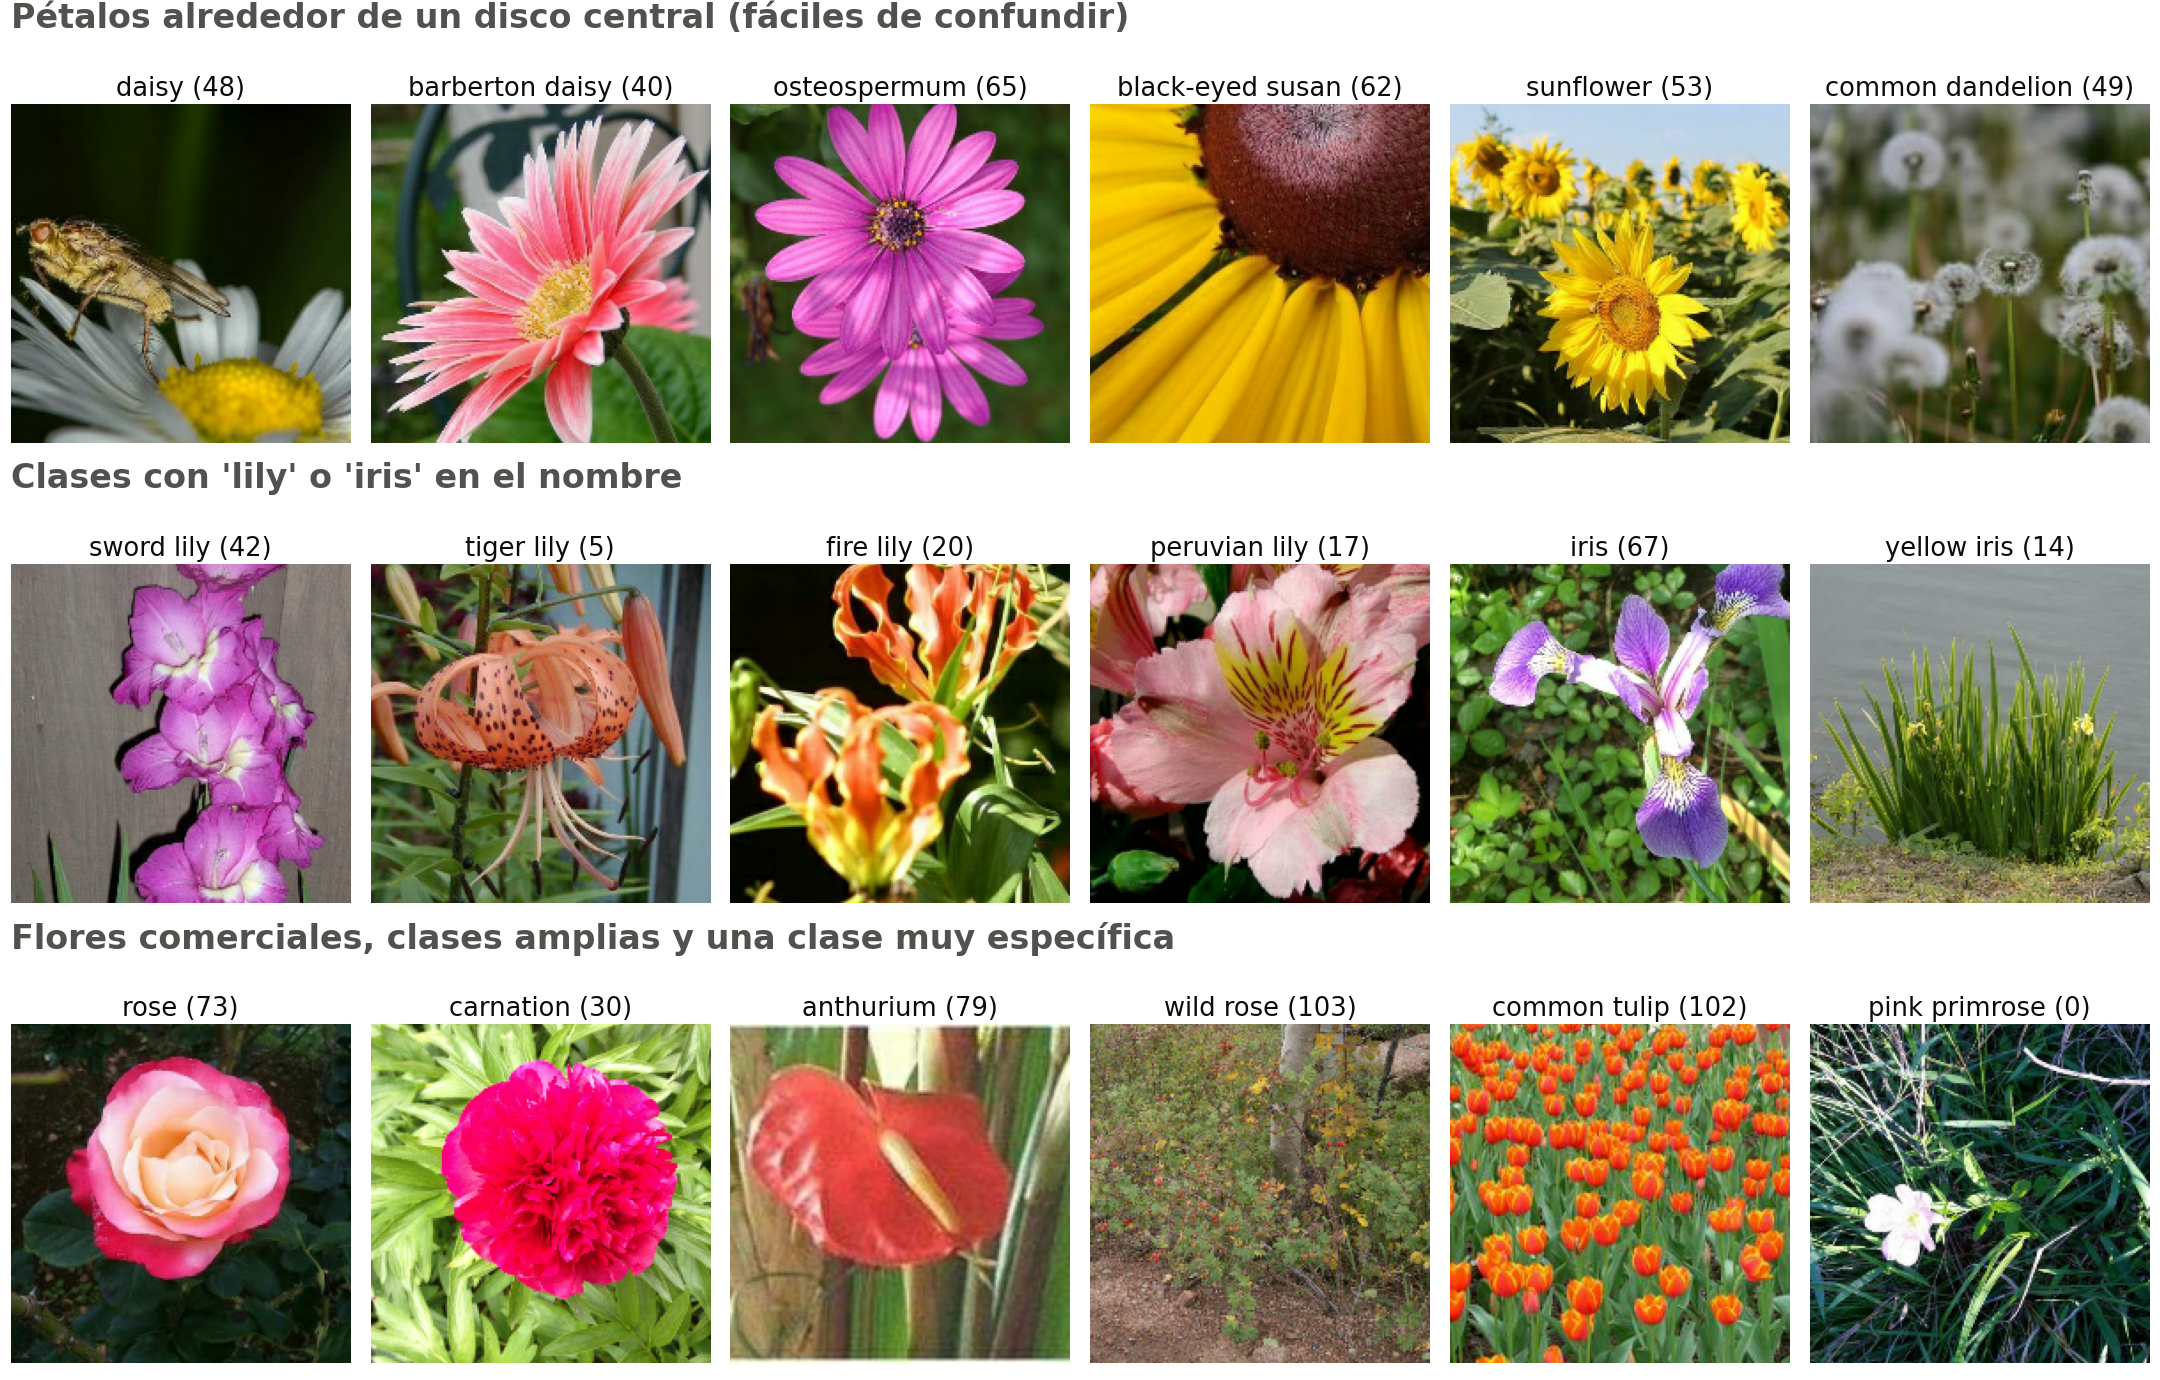
\includegraphics[width=\textwidth]{ejemplos_flores.png}
\caption{Ejemplos reales del conjunto de entrenamiento con su clase y número de etiqueta.}
\label{fig:ejemplos}
\end{figure*}

\begin{table*}[htbp]
\centering
\caption{Clases de ejemplo (nombre y etiqueta) y lo que ilustran.}
\label{tab:ejemplos}
\small
\begin{tabular}{p{0.35\textwidth}p{0.58\textwidth}}
\toprule
Clase (etiqueta) & Qué ilustra \\
\midrule
\textit{sunflower} (53) & Girasol. Flor grande y muy característica. Posiblemente sea de las más fáciles de identificar. \\
\textit{daisy} (48), \textit{barberton daisy} (40), \textit{osteospermum} (65), \textit{black-eyed susan} (62) & Margarita, gerbera, osteospermum y rudbeckia. Todas tienen pétalos alrededor de un disco central. Pueden surgir confusiones entre ellas. \\
\textit{sword lily} (42), \textit{tiger lily} (5), \textit{fire lily} (20), \textit{peruvian lily} (17) & Gladiola, lirio tigre, gloriosa y alstroemeria. Todas dicen \textit{lily}, pero son de cuatro familias botánicas distintas: el modelo tiene que fijarse en la forma, no en el nombre. \\
\textit{iris} (67), \textit{yellow iris} (14) & Misma forma general, la diferencia principal es el color. \\
\textit{rose} (73), \textit{wild rose} (103) & Dos clases de rosas. \textit{Wild rose} es amplia (varias subvariedades) y no viene de Oxford 102. \\
\textit{common tulip} (102) & Tulipán. Clase amplia que tampoco viene de Oxford 102. \\
\textit{pink primrose} (0) & Clase muy específica con un solo subtipo de flor. \\
\textit{carnation} (30) & Clavel, una de las flores comerciales que se producen en el Estado de México. \\
\bottomrule
\end{tabular}
\end{table*}

\subsection{Balance de clases y métrica de evaluación}
Con 12,753 imágenes de entrenamiento y 104 clases, tenemos en promedio 123 imágenes por clase ($12{,}753/104 \approx 122.6$). Sin embargo, las clases no tienen el mismo tamaño: como unas clases agrupan muchas subvariedades y otras solo una, algunas tienen muchas más imágenes que otras (de 18 a 782 imágenes de entrenamiento por clase).

Por este desbalance, la exactitud no basta: un modelo puede acertar mucho en las clases grandes, fallar en las clases pequeñas y aún verse bien. Por eso Kaggle califica con el F1 macro \parencite{kagglePetalsMetal}. Para cada clase $c$ se calcula la precisión $P_c$, la sensibilidad (\textit{recall}) $R_c$ y su media armónica:
\begin{equation}
P_c=\frac{TP_c}{TP_c+FP_c}, \quad R_c=\frac{TP_c}{TP_c+FN_c},
\end{equation}
\begin{equation}
F1_c=\frac{2\,P_c\,R_c}{P_c+R_c}, \qquad F1_{\text{macro}}=\frac{1}{104}\sum_{c=0}^{103}F1_c,
\end{equation}
donde $TP_c$, $FP_c$ y $FN_c$ son los verdaderos positivos, falsos positivos y falsos negativos de la clase $c$. Así, todas las clases pesan lo mismo, sin importar cuántas imágenes tengan.

\subsection{Implicaciones para el proyecto}
Como Kaggle ya separa entrenamiento y validación, no necesitamos hacer nuestra propia partición: entrenamos con \texttt{train}, elegimos modelos e hiperparámetros con \texttt{val} y reservamos \texttt{test} para la predicción final. Como las clases están desbalanceadas, siempre reportamos el F1 macro y no solo la exactitud.

\section{Algoritmos y aplicaciones}
Dado el problema planteado, su solución implica el uso de algoritmos de visión por computadora.

\subsection{Redes neuronales convolucionales (CNN)}
Las redes neuronales convolucionales (CNN) son una alternativa especialmente adecuada para este problema debido a su capacidad para procesar información espacial. Mediante filtros convolucionales pueden aprender automáticamente características de las imágenes, como bordes, texturas y formas (Figura~\ref{fig:cnn_diagram}). En las capas internas pueden emplearse funciones de activación como ReLU, mientras que Softmax puede utilizarse en la salida para representar las probabilidades de las distintas clases.

\begin{figure}[pos=!ht]
    \centering
    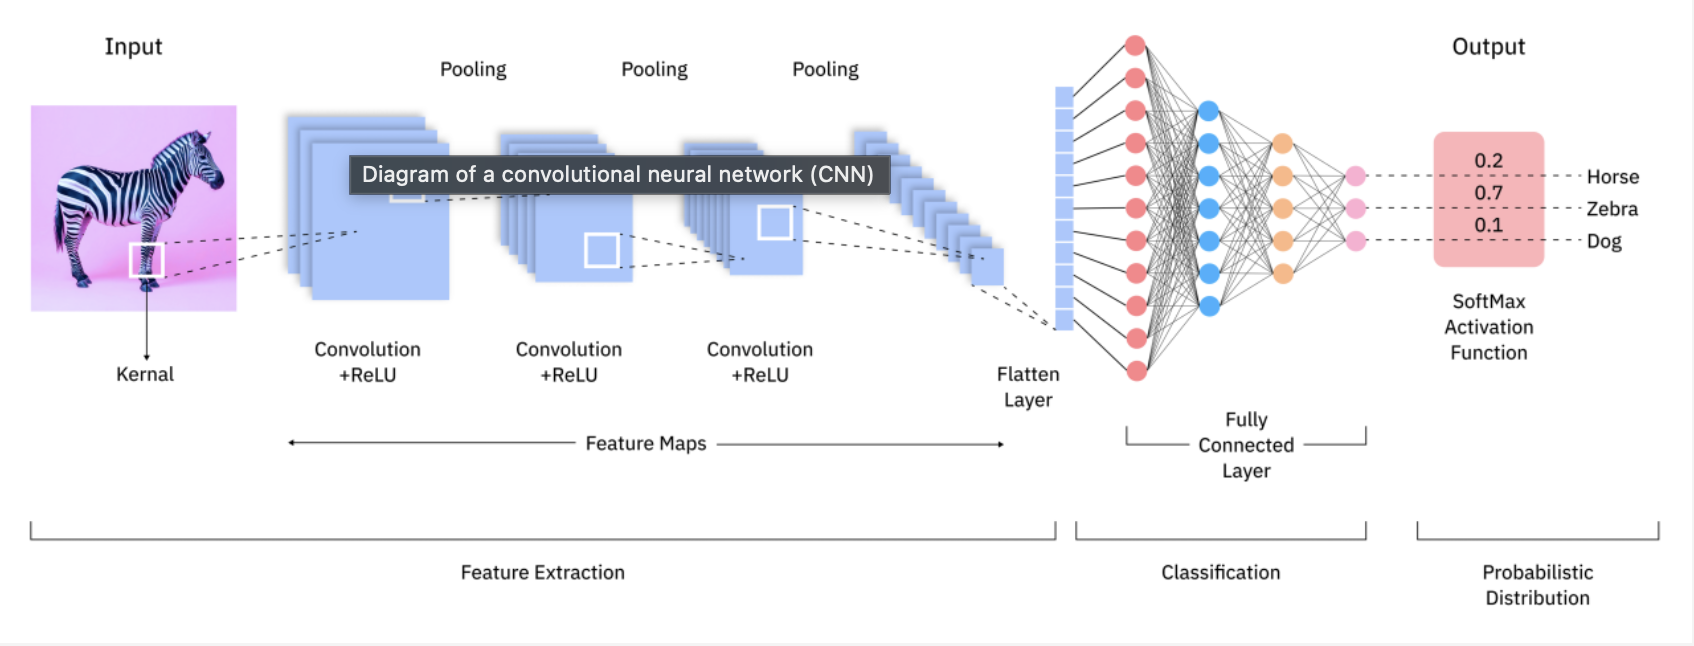
\includegraphics[width=\columnwidth]{cnn_diagram.png}
    \caption{La convolución descompone la imagen en características para aprender a clasificar \parencite{ibmWhatImage}.}
    \label{fig:cnn_diagram}
\end{figure}

Este método parece ser el más adecuado para obtener buenos resultados; sin embargo, por la cantidad de datos y de operaciones involucradas, es lento y computacionalmente pesado. Esto abre la posibilidad de usar otros algoritmos que se ajusten a las necesidades del problema.

\subsection{Otros algoritmos sin aprendizaje profundo}
\begin{description}
    \item[k vecinos más cercanos (KNN)] Representa cada imagen como un vector de características, mide la similitud entre puntos (normalmente con la distancia euclidiana) y clasifica la imagen según sus $k$ vecinos más cercanos. Es un algoritmo de aprendizaje supervisado.
    \item[Bosque aleatorio] Combina un conjunto de árboles de decisión y clasifica según el resultado de la mayoría de ellos.
    \item[Máquinas de vectores de soporte (SVM)] Encuentran el hiperplano óptimo para separar dos clases. La variante multiclase combina varios clasificadores binarios, como se requiere en este contexto.
\end{description}

\subsection{Otros modelos de aprendizaje profundo}
\begin{description}
    \item[ResNet] Conocida también como \textit{residual network}. Útil para entrenar redes neuronales muy profundas. Su principal limitante es la capacidad de nuestro \textit{hardware} o el acceso a equipo capaz de entrenar este tipo de redes.
    \item[Otros modelos ya implementados] Como \textbf{AlexNet} o \textbf{GoogLeNet/Inception}, que tienen una gran capacidad para reconocer y clasificar imágenes \parencite{ibmWhatImage}.
\end{description}

\subsection{Aplicaciones posibles}
Un modelo capaz de clasificar tipos de flores a partir de imágenes puede tener distintas aplicaciones reales. Una de ellas es la \textbf{identificación automática de plantas}, donde un usuario toma una fotografía y recibe como resultado la especie o clase más probable.

Un ejemplo de este tipo de aplicaciones está en el apoyo a plataformas de ciencia ciudadana y el monitoreo de biodiversidad. Por ejemplo, iNaturalist ha acumulado más de 300 millones de observaciones hechas por personas comunes \parencite{inaturalist} y utiliza un modelo de visión por computadora, entrenado con esas mismas observaciones, para sugerir la especie a partir de una fotografía. Sin este apoyo automático, cada observación dependería de que una persona la revisara detenidamente, lo que haría el proceso lento y difícil de escalar. Este proyecto es una versión a menor escala de este tipo de sistemas.

Otra aplicación sería como \textbf{herramienta educativa}, por ejemplo, en aplicaciones para estudiantes o visitantes de jardines botánicos que permitan reconocer flores y consultar información sobre ellas. Sin embargo, el modelo desarrollado solo podría reconocer las 104 clases presentes en el conjunto de datos, por lo que una aplicación real más amplia requeriría entrenarlo con una mayor variedad de especies.

\section{Metodología}

\subsection{Arquitectura de la red}
Para clasificar las 104 clases de flores se utiliza una red neuronal convolucional (CNN), ya que este tipo de red está diseñado para trabajar con imágenes y aprende automáticamente características espaciales como bordes, texturas, colores y formas.

Los experimentos se realizaron con imágenes RGB de $112\times112$ píxeles, obtenidas al redimensionar los archivos originales de $224\times224$; por tanto, la entrada de la red es de $112\times112\times3$. La Tabla~\ref{tab:arquitectura_cnn} resume la arquitectura. Se usan filtros de $3\times3$ porque analizan regiones pequeñas de la imagen: las primeras capas aprenden características simples, como bordes o cambios de color, y las posteriores las combinan para representar estructuras más complejas de las flores. El número de filtros aumenta de 32 a 256 mientras el \textit{max pooling} reduce el tamaño espacial.

\begin{table*}[htbp]
\centering
\caption{Arquitectura de la CNN (480,936 parámetros entrenables).}
\label{tab:arquitectura_cnn}
\small
\begin{tabular}{p{0.22\textwidth}p{0.46\textwidth}p{0.22\textwidth}}
\toprule
Capa & Configuración & Dimensión de salida \\
\midrule
Entrada & Imagen RGB & $112\times112\times3$ \\
Convolución 1 & 32 filtros de $3\times3$, \textit{padding same} + ReLU & $112\times112\times32$ \\
Max Pooling 1 & Ventana de $2\times2$ & $56\times56\times32$ \\
Convolución 2 & 64 filtros de $3\times3$, \textit{padding same} + ReLU & $56\times56\times64$ \\
Max Pooling 2 & Ventana de $2\times2$ & $28\times28\times64$ \\
Convolución 3 & 128 filtros de $3\times3$, \textit{padding same} + ReLU & $28\times28\times128$ \\
Max Pooling 3 & Ventana de $2\times2$ & $14\times14\times128$ \\
Convolución 4 & 256 filtros de $3\times3$, \textit{padding same} + ReLU & $14\times14\times256$ \\
Max Pooling 4 & Ventana de $2\times2$ & $7\times7\times256$ \\
Global Average Pooling & Promedio de cada mapa de características & 256 \\
Capa densa & 256 neuronas + ReLU & 256 \\
Dropout & Tasa de 0.5 & 256 \\
Salida & 104 neuronas (\textit{logits}), una por clase & 104 \\
\bottomrule
\end{tabular}
\end{table*}

\subsection{Preprocesamiento}
Cada registro TFRecord de $224\times224$ se decodifica como imagen RGB de tres canales, se redimensiona a $112\times112$ y se normaliza al intervalo $[0,1]$ mediante
\begin{equation}
x_{\text{norm}} = \frac{x}{255}.
\end{equation}
La reducción de resolución disminuye el costo de entrenamiento y conserva la forma y el color de las flores.

En el conjunto completo se aplica aumento de datos solo durante el entrenamiento: volteo horizontal, rotación de hasta $\pm18^\circ$, acercamiento o alejamiento de hasta 10\,\% y variación de contraste de hasta 10\,\%. Estas transformaciones generan versiones distintas de una misma imagen sin modificar su clase. A validación y prueba no se les aplica ninguna transformación aleatoria, para evaluar siempre las mismas imágenes.

\subsection{Función de pérdida y entrenamiento}
Cada imagen pertenece a una sola de las 104 clases, por lo que se utiliza la entropía cruzada categórica dispersa. La red produce 104 \textit{logits} $z_k$, que Softmax convierte en probabilidades:
\begin{equation}
\hat{y}_k = \frac{e^{z_k}}{\sum_{j=1}^{104} e^{z_j}}.
\end{equation}
Para una imagen de clase $c$, la pérdida es $L = -\log(\hat{y}_c)$: es pequeña si el modelo asigna alta probabilidad a la clase correcta y grande si se equivoca con confianza. Se usa la versión dispersa porque las etiquetas son enteros de 0 a 103 y no hace falta convertirlas a vectores \textit{one-hot}.

Los gradientes se calculan con retropropagación y los parámetros se actualizan con Adam, con una tasa de aprendizaje de $10^{-3}$ y minilotes de 32 imágenes mezcladas en cada época. Después de cada evaluación se calcula el F1 macro de validación, se guarda el modelo con el mejor F1 (\textit{checkpoint}) y el entrenamiento se detiene tras cinco evaluaciones consecutivas sin mejora (parada temprana).

\subsection{Destilación de datos mediante Distribution Matching}
Además del entrenamiento convencional, se implementó la destilación de datos mediante \textit{Distribution Matching} (DM) \parencite{zhao2023dm}. Su objetivo es generar un conjunto reducido de imágenes sintéticas que conserve las características representativas del conjunto original.

El método utiliza una red convolucional como extractor de características. En cada iteración se inicializan nuevos pesos aleatorios y se obtienen las representaciones de imágenes reales y sintéticas de cada clase. La función objetivo minimiza la distancia cuadrática entre los promedios de estas representaciones:
\begin{equation}
L_{DM} = \sum_{c=0}^{103} \left\lVert \mu_c^{\text{real}} - \mu_c^{\text{sint}} \right\rVert_2^2,
\end{equation}
donde $\mu_c^{\text{real}}$ y $\mu_c^{\text{sint}}$ son los vectores promedio de características de las imágenes reales y sintéticas de la clase $c$. Solo se optimizan los píxeles de las imágenes sintéticas; los pesos del extractor permanecen fijos durante cada paso.

Se utilizó Adam con una tasa de aprendizaje de 0.01 sobre los píxeles durante 500 iteraciones completas, con transformaciones diferenciables de aumento de datos (DSA) \parencite{zhao2021dsa} sobre las imágenes reales y sintéticas. Se generaron conjuntos de una y diez imágenes por clase (IPC = 1 e IPC = 10), que después se usaron para entrenar la CNN; durante ese entrenamiento también se aplica DSA.

\section{Entrenamiento y resultados}
En esta etapa se entrenó la CNN con el conjunto completo y se evaluó el efecto de reducir el número de imágenes disponibles por clase, comparando subconjuntos aleatorios de fotografías reales con conjuntos sintéticos obtenidos con DM. Después, con el conjunto completo, se probaron variaciones de hiperparámetros. Todas las tablas y figuras de esta sección se generan con el notebook \texttt{reports/entregable\_3/avance3.ipynb} del repositorio público del proyecto \parencite{repositorio} (sección~\ref{sec:notebook}).

\subsection{Diseño de los experimentos}
Se consideraron tres modalidades de entrenamiento. La primera, \textit{conjunto completo}, emplea las 12,753 imágenes reales de entrenamiento y funciona como referencia. La segunda, \textit{aleatorio}, utiliza un subconjunto balanceado de fotografías reales tomadas al azar, con la misma cantidad de imágenes por clase. La tercera, \textit{destilado}, sustituye ese subconjunto por imágenes sintéticas optimizadas con DM. En las dos últimas se evaluaron dos tamaños: una imagen por clase (IPC = 1, 104 imágenes) y diez imágenes por clase (IPC = 10, 1,040 imágenes), que representan reducciones del 99.18\,\% y 91.85\,\% frente al conjunto original.

Las cuatro configuraciones reducidas se entrenaron con las semillas 0, 1 y 2, hasta 300 épocas, evaluando validación cada diez épocas. El conjunto completo se entrenó una vez (semilla 0), hasta 50 épocas, evaluando validación en cada época. En todos los casos se usó el mismo conjunto de validación de 3,712 imágenes reales; los datos de prueba no se usaron para seleccionar modelos.

\subsection{Resultados de clasificación}
La Tabla~\ref{tab:resultados} resume los resultados. Para los conjuntos reducidos se presenta el promedio de las tres semillas y la desviación estándar muestral del F1 macro. La exactitud se incluye como métrica complementaria, pero el F1 macro es la medida principal por el desbalance entre clases.

\begin{table*}[htbp]
\centering
\caption{Resultados de validación y tiempo de entrenamiento de la CNN a $112\times112$. Para los conjuntos reducidos se reportan promedios de tres semillas.}
\label{tab:resultados}
\small
\begin{tabular}{lcccrr}
\toprule
Modalidad & IPC & Corridas & F1 macro & Exactitud (\%) & Entrenamiento (s) \\
\midrule
Aleatorio & 1 & 3 & 0.0514 $\pm$ 0.0029 & 5.75 & 35.4 \\
Destilado (DM) & 1 & 3 & 0.0672 $\pm$ 0.0052 & 9.85 & 36.3 \\
Aleatorio & 10 & 3 & 0.2575 $\pm$ 0.0082 & 25.86 & 329.4 \\
Destilado (DM) & 10 & 3 & 0.2044 $\pm$ 0.0235 & 20.55 & 272.5 \\
Conjunto completo & -- & 1 & 0.5538 & 61.61 & 581.5 \\
\bottomrule

\end{tabular}
\end{table*}

Con una sola imagen por clase, el conjunto destilado alcanzó un F1 macro promedio de 0.0672, frente a 0.0514 con imágenes reales elegidas al azar, una diferencia de 0.0158 a favor de DM. Esto sugiere que, con una reducción extrema, la optimización de las imágenes sintéticas conserva información útil para la clasificación. Con diez imágenes por clase ocurrió lo contrario: la selección aleatoria alcanzó 0.2575 y el conjunto destilado 0.2044, una diferencia de 0.0531 a favor de las fotografías reales (Figura~\ref{fig:comparacion}). Por tanto, la destilación no mostró una ventaja consistente en ambos tamaños.

La CNN entrenada con el conjunto completo obtuvo el mejor resultado: F1 macro de 0.5538 y exactitud de 61.61\,\%. Como el modelo completo se entrenó una sola vez y las demás configuraciones cuentan con tres repeticiones, estas comparaciones son resultados preliminares, no evidencia estadística definitiva.

\begin{figure}[pos=!ht]
\centering
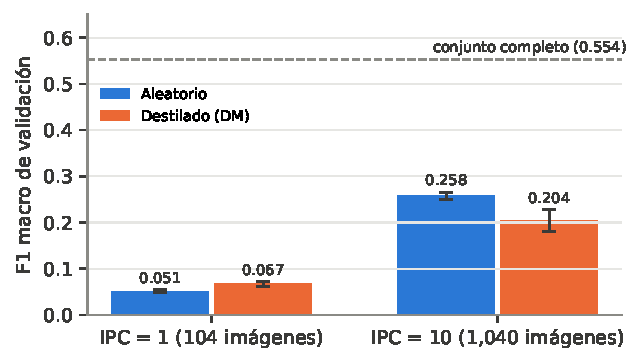
\includegraphics[width=\columnwidth]{comparacion_f1.pdf}
\caption{F1 macro de validación de los subconjuntos aleatorios y destilados. Las barras de error indican una desviación estándar entre tres semillas y la línea discontinua, la corrida con el conjunto completo.}
\label{fig:comparacion}
\end{figure}

\subsection{Costo computacional de la destilación}
La Tabla~\ref{tab:costos} separa el tiempo de entrenamiento del tiempo de destilación. Los tiempos de entrenamiento excluyen las evaluaciones periódicas de validación. La destilación se ejecutó una sola vez por IPC y sus imágenes se reutilizaron en las tres semillas, por lo que no debe contarse una destilación por semilla. La columna ``Total'' suma una destilación al tiempo promedio de entrenamiento; estima el costo de preparar el conjunto sintético y entrenar un modelo con él, pero no incluye la descarga ni la preparación de los datos.

\begin{table}[htbp]
\centering
\caption{Tiempo promedio de entrenamiento y de destilación previa, en segundos.}
\label{tab:costos}
\small
\begin{tabular}{lcrrr}
\toprule
Modalidad & IPC & Entren. & Destil. & Total \\
\midrule
Aleatorio & 1 & 35.4 & -- & 35.4 \\
Destilado (DM) & 1 & 36.3 & 985.4 & 1,021.7 \\
Aleatorio & 10 & 329.4 & -- & 329.4 \\
Destilado (DM) & 10 & 272.5 & 1,510.0 & 1,782.5 \\
Conjunto completo & -- & 581.5 & -- & 581.5 \\
\bottomrule

\end{tabular}
\end{table}

Aunque entrenar con conjuntos reducidos toma menos tiempo que usar las 12,753 fotografías, la destilación incrementa considerablemente el costo inicial: con IPC = 10, preparar y entrenar el conjunto destilado (1,782.5 s) toma más que entrenar con el conjunto completo (581.5 s). Por ello, los resultados no permiten concluir que DM sea más rápido para entrenar un solo modelo; su costo solo podría amortizarse si las mismas imágenes sintéticas se reutilizaran en muchos entrenamientos.

\subsection{Curvas de aprendizaje}
Cada corrida guarda un archivo \texttt{history.csv} con la pérdida y la exactitud de entrenamiento y la pérdida, exactitud y F1 macro de validación por época. Las métricas de entrenamiento se registran durante la época, con aumento de datos y \textit{dropout} activos, mientras que las de validación se calculan al final de la época sin transformaciones. Por eso, al inicio, la exactitud de validación puede ser mayor que la de entrenamiento.

\paragraph{Conjunto completo.} La Figura~\ref{fig:curvas_completo} muestra que las pérdidas de entrenamiento y validación bajan juntas hasta la época 21 (de 3.94 y 3.59 a 1.69 y 1.74). A partir de la época 25 se separan: la de entrenamiento sigue bajando hasta 1.07, mientras que la de validación se estanca entre 1.51 y 1.69. La exactitud muestra lo mismo: al final, la de entrenamiento llega a 68.1\,\% y la de validación se queda en 62.6\,\%. Es el inicio del sobreajuste, aunque moderado, porque el F1 de validación todavía mejora lentamente hasta la época 38 (0.5538), que coincide con la menor pérdida de validación (1.510). En las cinco épocas siguientes el F1 no mejoró, y la parada temprana detuvo el entrenamiento en la época 43. El \textit{checkpoint} guardado corresponde a la época 38, así que el modelo reportado no incluye las épocas en las que empezaba a sobreajustar.

\begin{figure*}[htbp]
\centering
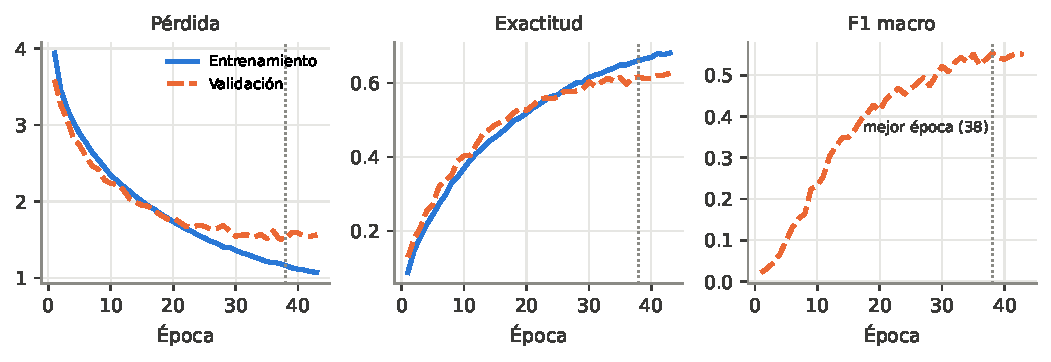
\includegraphics[width=0.9\textwidth]{curvas_completo.pdf}
\caption{Curvas de aprendizaje con el conjunto completo: pérdida y exactitud de entrenamiento frente a validación, y F1 macro de validación. La línea punteada marca la mejor época (38), cuyo modelo se guardó.}
\label{fig:curvas_completo}
\end{figure*}

\paragraph{Conjuntos reducidos.} En la Figura~\ref{fig:curvas_reducidos}, el sobreajuste es mucho más marcado. Con IPC = 10, la exactitud de entrenamiento llega a 70--85\,\% y la pérdida de entrenamiento baja a 0.5--0.9, pero la exactitud de validación se estanca alrededor de 25\,\% (aleatorio) y 19\,\% (destilado). La pérdida de validación alcanza su mínimo entre las épocas 30 y 50 (alrededor de 3.6--3.9) y luego crece hasta 7.4--9.3, es decir, la red memoriza las 1,040 imágenes. Con IPC = 1 ocurre lo mismo con mayor intensidad: la validación queda entre 5 y 10\,\% de exactitud y su pérdida sube hasta 12--18. El conjunto destilado con IPC = 1 se ajusta más lentamente (exactitud de entrenamiento final de 57--63\,\%, contra 62--83\,\% del aleatorio), lo que concuerda con que sus imágenes sintéticas resumen la clase en lugar de ser ejemplos fáciles de memorizar.

Aunque la pérdida de validación crece, el mejor F1 de los conjuntos reducidos se alcanza tarde (entre las épocas 170 y 280). Esto pasa porque la pérdida castiga las predicciones equivocadas hechas con mucha confianza, mientras que el F1 solo depende de la clase predicha: el modelo sigue acertando algunas imágenes más, pero se vuelve muy confiado en sus errores. Por eso conviene seleccionar el modelo por F1 y no por la pérdida.

\begin{figure*}[htbp]
\centering
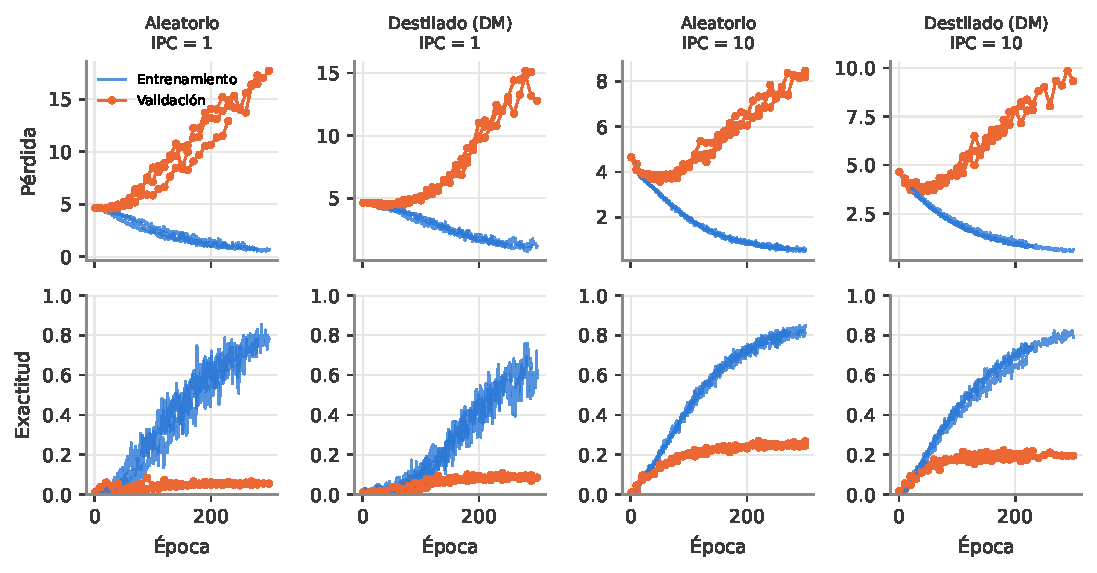
\includegraphics[width=0.95\textwidth]{curvas_reducidos.pdf}
\caption{Curvas de aprendizaje de los conjuntos reducidos (tres semillas por configuración). Validación se evaluó cada diez épocas; los marcadores indican las épocas evaluadas.}
\label{fig:curvas_reducidos}
\end{figure*}

\subsection{Experimentos de hiperparámetros con el conjunto completo}
Para estudiar los hiperparámetros, se tomó como referencia una política de entrenamiento con AdamW (\textit{weight decay} de 0.01), tasa de aprendizaje inicial de $10^{-3}$ que se reduce a la mitad cuando la pérdida de validación se estanca, \textit{dropout} de 0.5, aumento de datos, lotes de 64 y paciencia de 12 épocas. A partir de ella se cambió \textbf{un solo factor} en cada experimento: la tasa de aprendizaje ($3\times10^{-4}$), el \textit{dropout} (0.3) y la regularización en conjunto (sin \textit{dropout}, sin aumento de datos y sin \textit{weight decay}). En estas corridas, las métricas de entrenamiento se miden sobre 3,712 imágenes fijas de entrenamiento sin aumentos ni \textit{dropout}, igual que validación, por lo que la brecha entre ambas sí mide el sobreajuste. Los resultados están en la Tabla~\ref{tab:hiperparametros} y la Figura~\ref{fig:curvas_hp}.

\begin{table*}[htbp]
\centering
\caption{Efecto de los hiperparámetros con el conjunto completo (una semilla). La brecha es el F1 de entrenamiento menos el de validación en la mejor época.}
\label{tab:hiperparametros}
\small
\begin{tabular}{lrrrrc}
\toprule
Configuración & F1 val. & Exactitud val. (\%) & F1 entren. & Brecha & Mejor época / épocas \\
\midrule
Referencia (LR $10^{-3}$, dropout 0.5) & 0.5784 & 64.06 & 0.814 & 0.235 & 91 / 103 \\
Tasa de aprendizaje $3\times10^{-4}$ & 0.4605 & 54.18 & 0.554 & 0.094 & 98 / 110 \\
Dropout 0.3 & 0.5596 & 61.96 & 0.816 & 0.256 & 61 / 73 \\
Sin dropout, aumento ni weight decay & 0.5332 & 59.64 & 0.877 & 0.344 & 34 / 46 \\
\bottomrule

\end{tabular}
\end{table*}

\begin{figure*}[htbp]
\centering
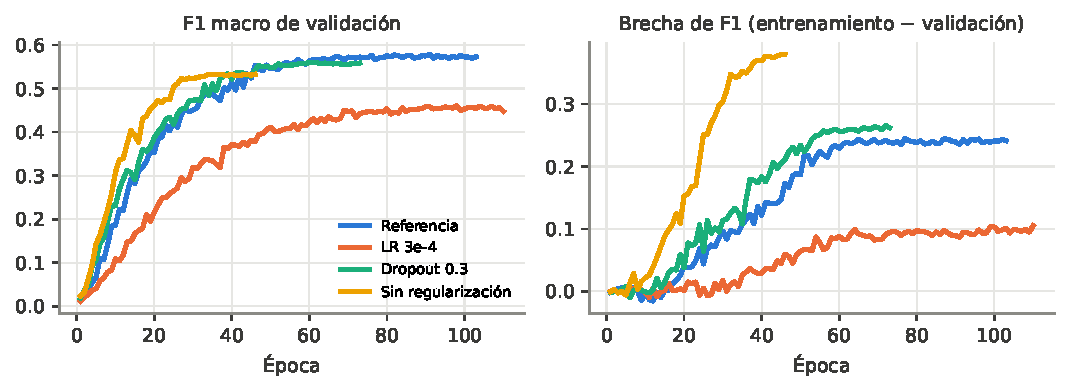
\includegraphics[width=0.9\textwidth]{curvas_hiperparametros.pdf}
\caption{F1 macro de validación y brecha de F1 entre entrenamiento y validación por época para cada configuración de hiperparámetros.}
\label{fig:curvas_hp}
\end{figure*}

\paragraph{Tasa de aprendizaje.} Reducir la tasa de $10^{-3}$ a $3\times10^{-4}$ bajó el F1 de 0.5784 a 0.4605. La brecha es la más pequeña (0.094), pero el F1 de entrenamiento también es bajo (0.554): el modelo no está sobreajustando, está \textbf{subajustando}. Con pasos más pequeños, la red aprende más lento y la reducción automática de la tasa la lleva al mínimo ($10^{-5}$) antes de converger, así que después de 110 épocas sigue lejos de la referencia. Con este presupuesto de épocas, $10^{-3}$ es la mejor opción.

\paragraph{Dropout.} Bajar el \textit{dropout} de 0.5 a 0.3 redujo el F1 a 0.5596 y aumentó ligeramente la brecha (de 0.235 a 0.256). La menor pérdida de validación también empeoró (de 1.464 a 1.596). Con menos neuronas apagadas, la capa densa memoriza un poco más, así que conviene mantener 0.5.

\paragraph{Regularización.} Sin \textit{dropout}, sin aumento de datos y sin \textit{weight decay}, la red converge más rápido (mejor época 34 de 46), pero alcanza la brecha más grande (0.344): el F1 de entrenamiento llega a 0.877, mientras que el de validación se queda en 0.5332. Es el caso más claro de \textbf{sobreajuste}, lo que confirma que la regularización es la responsable de la mejora de la referencia.

La referencia (F1 de 0.5784, exactitud de 64.06\,\%) supera a la corrida original del Avance 3 (0.5538). Sin embargo, como esa política cambia varios factores a la vez (optimizador, reducción de la tasa, tamaño de lote y paciencia), la mejora no puede atribuirse a uno solo. No se evaluó el tamaño de imagen; queda como siguiente experimento, por ejemplo $160\times160$.

\subsection{Notebook y reproducibilidad}
\label{sec:notebook}
El notebook \texttt{reports/entregable\_3/avance3.ipynb} del repositorio \url{https://github.com/Lunaaaalj/NeuralNetworksTeamEnvironment} reproduce esta sección de principio a fin: descarga y revisión de los datos, construcción de la CNN, entrenamiento de todas las configuraciones (activando \texttt{RUN\_TRAINING}), re-evaluación de los modelos guardados, generación de las Tablas~\ref{tab:resultados}, \ref{tab:costos} y~\ref{tab:hiperparametros} y de todas las figuras de curvas. La configuración exacta del Avance 3 está en \texttt{config\_avance3.yaml} y la de cada experimento de hiperparámetros, junto con su historial, en \texttt{hiperparametros/}. Al re-evaluar los 13 modelos guardados sobre las 3,712 imágenes de validación, el F1 macro y la exactitud coincidieron exactamente con los registrados durante el entrenamiento.

\subsection{Limitaciones y siguientes pasos}
El tamaño y la composición del conjunto de entrenamiento influyen mucho en el desempeño de la CNN. DM mejoró a la selección aleatoria con una imagen por clase, pero no con diez, y el costo de crear las imágenes sintéticas superó el de entrenar con ellas. Con el conjunto completo, la regularización (\textit{dropout} de 0.5, aumento de datos y \textit{weight decay}) y una tasa de aprendizaje de $10^{-3}$ dieron el mejor resultado.

Las conclusiones están limitadas a una arquitectura, una resolución de $112\times112$, una sola semilla en los experimentos con el conjunto completo y al conjunto de validación, ya que las etiquetas de prueba no están disponibles. Los siguientes pasos son probar resoluciones mayores, repetir los experimentos de hiperparámetros con varias semillas y estudiar qué clases son más difíciles de reconocer.


\printbibliography[title=Referencias]
\end{document}
